\section{Апробация машинного обучения}
В данной главе описывается апробирование подхода к анализу систем массового обслуживания при помощи машинного обучения, а именно --- предсказывание коэффициента вариации длин интервалов между моментами покидания заявок системы. Данный метод широко используется во многих других областях науки и является универсальным: подходит для задач регрессии, временных рядов, а также классификации и кластеризации \cite{libbrecht2015machine,shinde2018review,soofi2017classification}. В теории массового обслуживания также есть примеры исследования, в которых успешно используется машинное обучение \cite{ojeda2021learning,xue2016scheduling,balla2018reliability}.

\subsection{Разведочный анализ}
В данном случае машинное обучение будет использоваться для решения задачи регрессии. Для этой цели, при помощи ранее описанных инструментов, было проведено около 286 тысяч запусков имитационной модели при различных параметрах входящего потока, орбиты и обслуживающего прибора для создания выборки, на основе которой и будет решена задача.

Исходная выборка имеет 9 признаков:
\begin{enumerate}
	\item elapsed --- время работы имитационной модели в секундах. Данный признак был добавлен в утилитарных целях, в частности, для последующей оптимизации работы модели при нестандартных параметрах. Действительное число.
	\item mean\_input --- среднее число обслуженных заявок входящего потока за интервал моделирования. Действительное число.
	\item var --- коэффициент вариации длин интервалов между моментами наступления событий во входящем потоке. Действительное число.
	\item alpha --- интенсивность вызова заявок прибором ($\alpha$). Действительное число.
	\item lg --- интенсивность входящего потока \eqref{eq_lg}. Действительное число.
	\item mu1 --- интенсивность обслуживания входящих заявок ($\mu_1$). Действительное число.
	\item mu2 --- интенсивность обслуживания вызванных заявок ($\mu_2$). Действительное число.
	\item sigma --- интенсивность обращений заявок с орбиты ($\sigma$). Действительное число.
	\item var\_input --- коэффициент вариации выходящего процесса. Действительное число. Является целевой переменной для предсказаний.
\end{enumerate}

Все признаки имеют 270420 (часть экспериментов выбыли из-за превышения временного лимита на выполнение) ненулевых значений и распределены следующим образом	
\begin{table}[H]
	\centering
	\caption{Распределение признаков}
	\label{table_feature_distr}
\begin{tabular}{|l|l|l|l|l|l|l|l|l|l|l|}
\hline
	  & elapsed & mean\_input & var\_input &     alpha &        lg &       mu1 &       mu2 &     sigma &       var \\
\hline
	mean & 7.36 &       5.52 & 1.11 &      1.26 &      1.90 &      2.97 &      2.71 &      1.41 &      1.32 \\
\hline
	std & 23.16 &       5.43 & 0.20 &      0.91 &      0.68 &      0.66 &      0.81 &      0.86 &      0.31 \\
\hline
	min & 0.01 &       0.00 & 0.71 &      0.00 &      1.00 &      1.20 &      1.00 &      0.01 &      1.00 \\
\hline
	10\% & 0.79 &       0.57 & 0.93 &      0.20 &      1.00 &      2.00 &      1.40 &      0.21 &      1.05 \\
\hline
	20\% & 1.29 &       1.15 & 1.00 &      0.40 &      1.20 &      2.40 &      2.00 &      0.61 &      1.09 \\
\hline
	30\% & 1.74 &       1.82 & 1.01 &      0.60 &      1.40 &      2.60 &      2.20 &      0.81 &      1.14 \\
\hline
	40\% & 2.19 &       2.66 & 1.03 &      0.80 &      1.60 &      2.80 &      2.60 &      1.21 &      1.18 \\
\hline
	50\% & 2.70 &       3.70 & 1.06 &      1.20 &      1.80 &      3.00 &      2.80 &      1.41 &      1.24 \\
\hline
	60\% & 3.34 &       5.03 & 1.09 &      1.40 &      2.00 &      3.20 &      3.00 &      1.81 &      1.30 \\
\hline
	70\% & 4.32 &       6.77 & 1.14 &      1.80 &      2.20 &      3.40 &      3.20 &      2.01 &      1.37 \\
\hline
	80\% & 6.21 &       9.23 & 1.20 &      2.00 &      2.60 &      3.60 &      3.60 &      2.41 &      1.48 \\
\hline
	90\% & 11.76 &      13.25 & 1.32 &      2.60 &      2.80 &      3.80 &      3.80 &      2.61 &      1.67 \\
\hline
	95\% & 22.72 &      16.87 & 1.46 &      3.00 &      3.20 &      3.80 &      3.80 &      2.81 &      1.87 \\
\hline
	99\% & 104.70 &      24.02 & 1.86 &      3.40 &      3.40 &      3.80 &      3.80 &      2.81 &      2.45 \\
\hline
	max & 419.53 &      35.89 & 5.99 &      3.60 &      3.60 &      3.80 &      3.80 &      2.81 &      8.19 \\
\hline
\end{tabular}
\end{table}
На основе сводки из таблицы \ref{table_feature_distr} можно заметить, что в среднем время моделирования занимало 7.36 секунд, половина экспериментов была запущена с интенсивностью входящего потока 1.8, а максимальный коэффициент вариации выходящего процесса составил 8.19.



На данном этапе мы можем избавиться от признаков, которые не будут участвовать в обучении модели: mean\_input и elapsed. Для оставшихся признаков построим графики рассеяния \cite{cox2007pairplot}. Данные диаграммы полезны для отображения многомерных данных, как в данном случае. С их помощью можно определить потенциальные взаимосвязи между количественными переменными.
\begin{figure}[H]
	\centering
	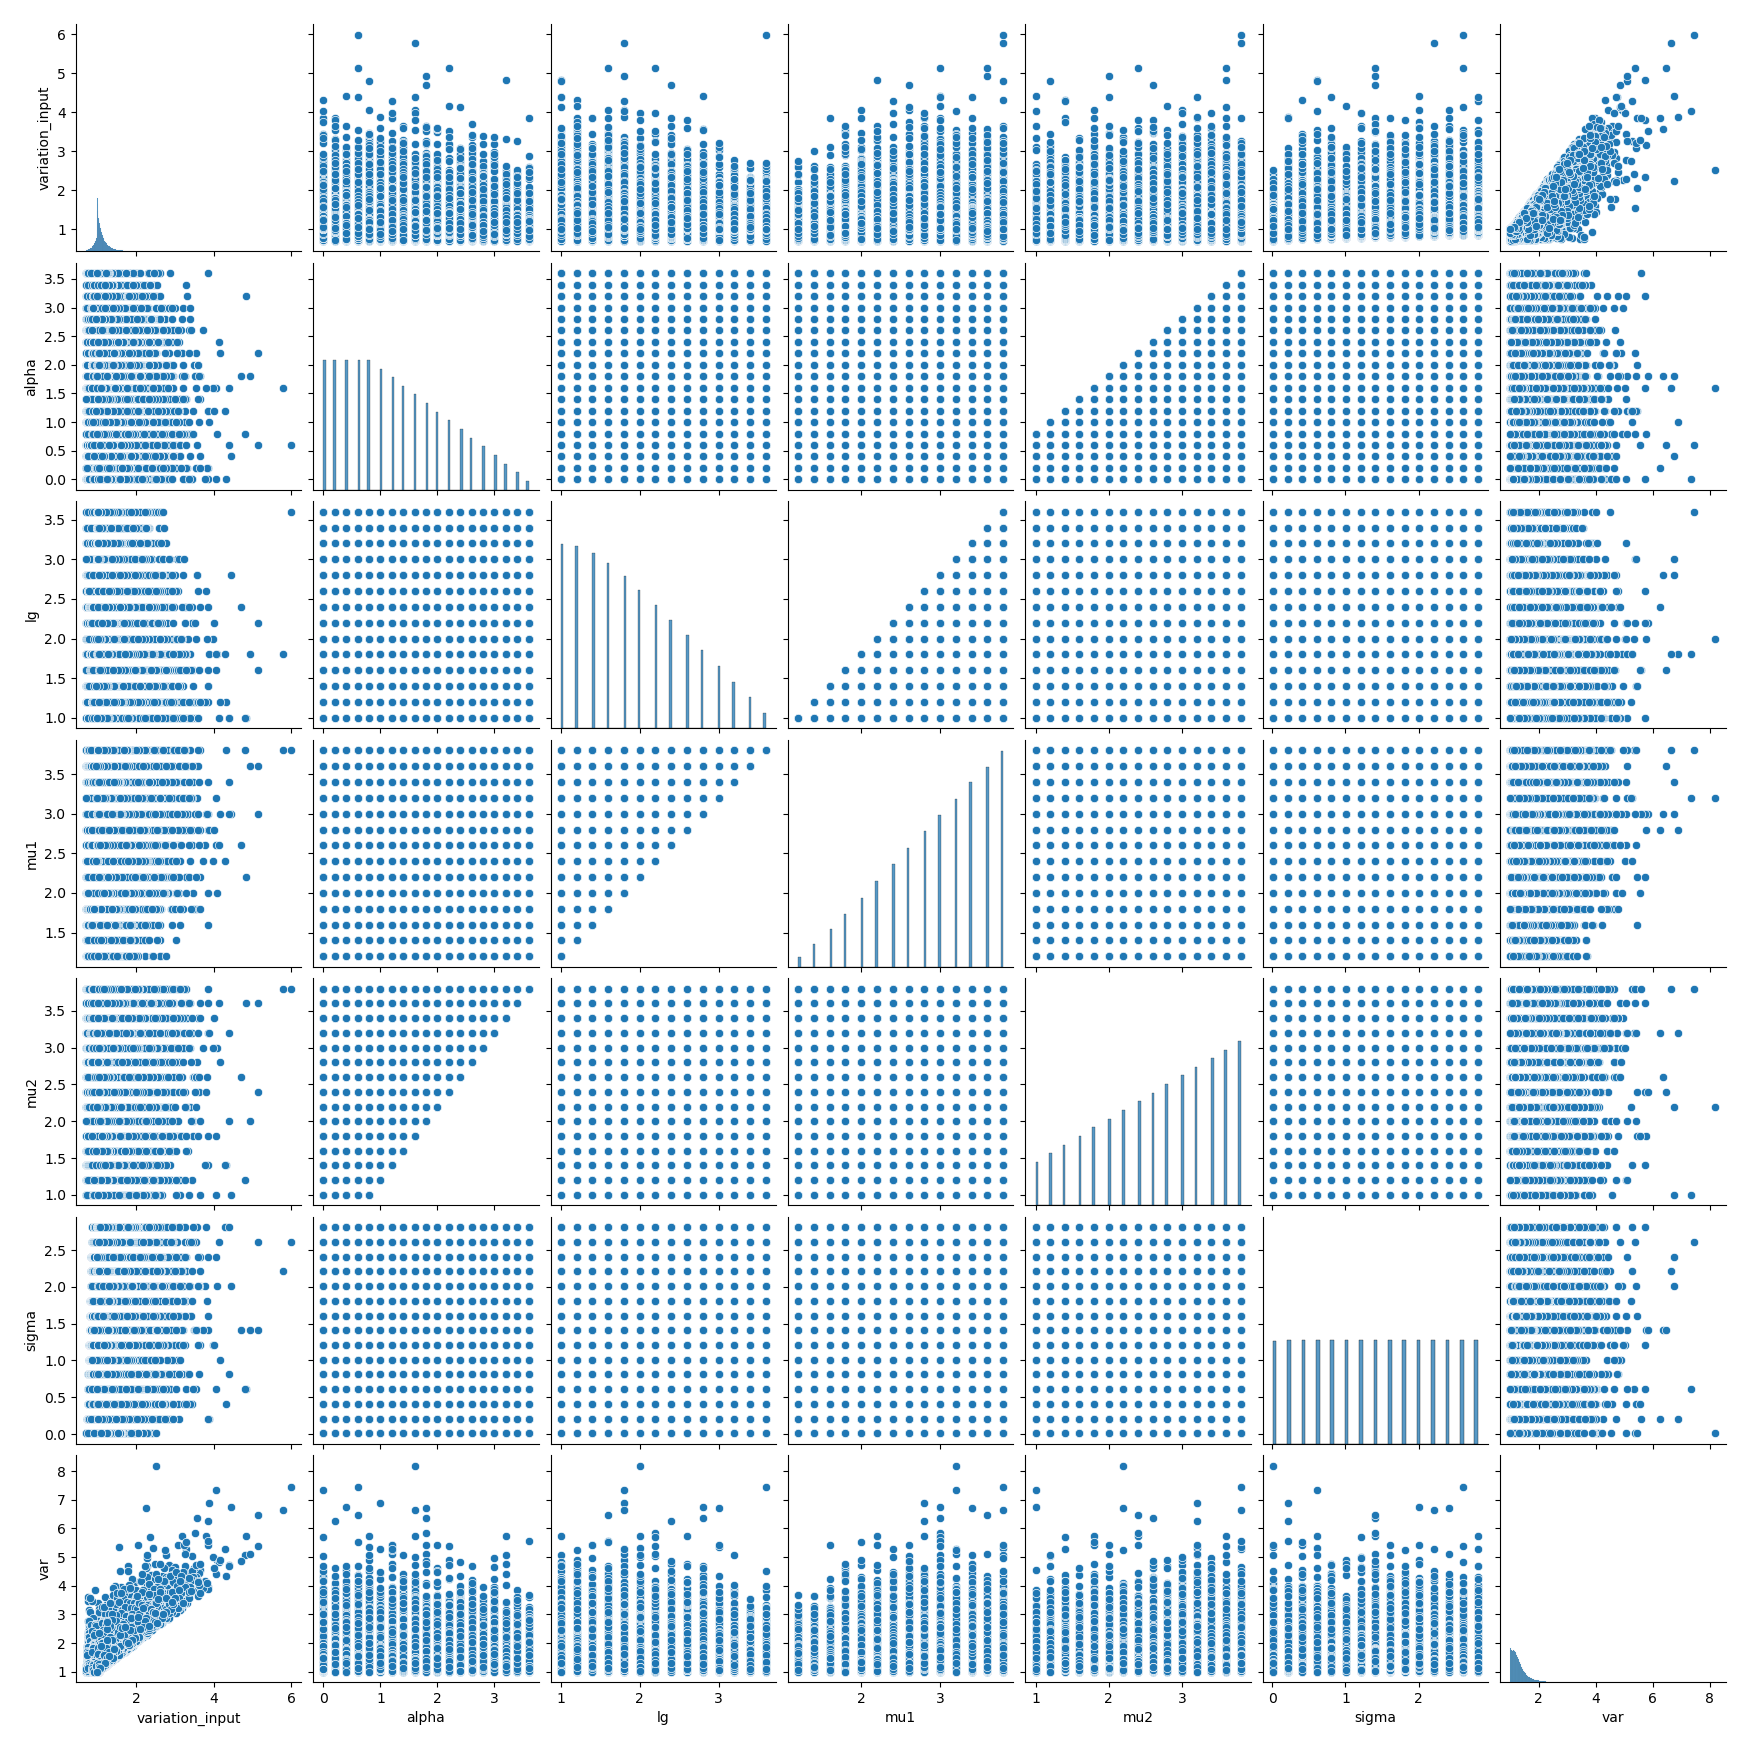
\includegraphics[scale=0.8,width=\textwidth]{pairplot.png}
	\caption{Графики рассеяния признаков}
	\label{pairplot}
\end{figure}
\clearpage
На графике рассеяния \ref{pairplot} видно, что явную связь имеют коэффициент вариации входящего потока (var) и коэффициент вариации выходящего процесса (var\_input). Для более точного определения зависимостей построим для признаков тепловую карту коэффициента корреляции Пирсона
\begin{figure}[H]
	\centering
	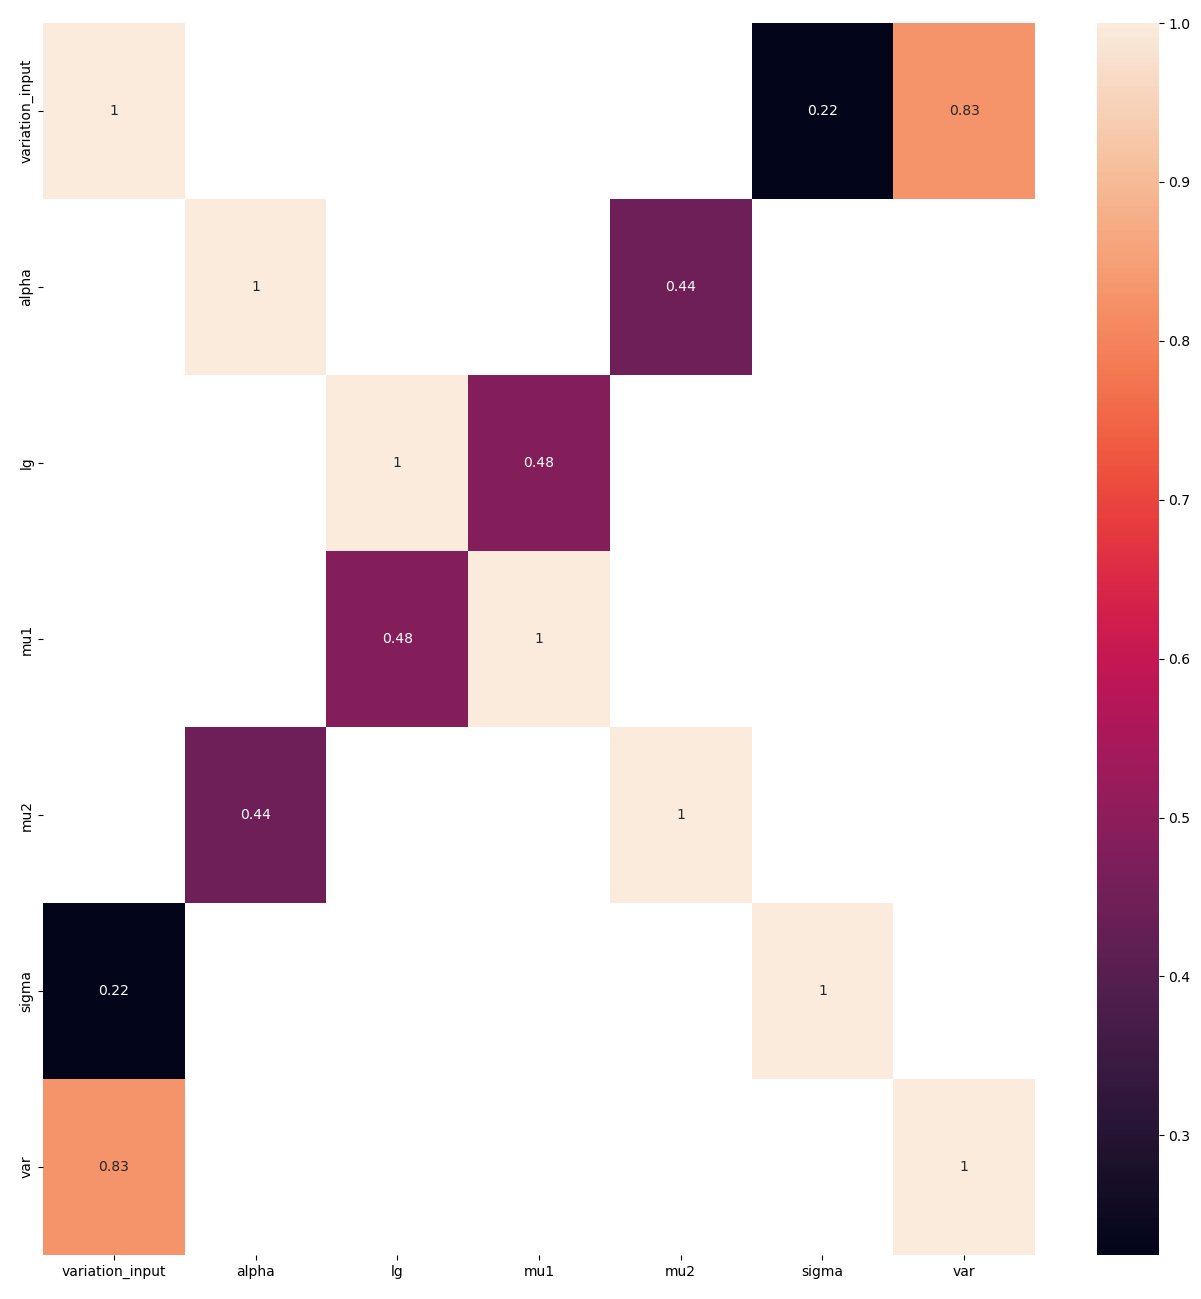
\includegraphics[scale=0.8,width=\textwidth]{pearson_heatmap.png}
	\caption{Тепловая карта корреляции признаков}
	\label{pearson_heatmap}
\end{figure}
На рисунке \ref{pearson_heatmap} можно наблюдать логичную корреляцию таких признаков, как интенсивность обслуживания входящих заявок (mu1) и интенсивность входящего потока (lg), а также интенсивность обслуживания вызванных заявок (mu2) и интенсивность их вызова (alpha). Для целевой переменной же можно наблюдать ранее выявленную корреляцию с коэффициентом вариации входящего потока и интенсивностью обращения заявок с орбиты (sigma), что так же ожидаемо, поскольку задержка заявок на орбите влияет на пропускную способность прибора.

\subsection{Построение предсказательных моделей}
Для настройки и обучения предсказательных моделей используется язык Python и библиотека для ансамблевого машинного обучения scikit-learn \cite{hackeling2017mastering}. Ансамблевые методы машинного обучения являются мощным и в то же время простым для понимая инструментом анализа данных. Он представляет собой метод обучения, где несколько моделей обучаются решению одной и той же задачи и объединяются для получения наиболее точных результатов. Ключевое преимущество такого метода заключается в том, что результат работы нескольких моделей будет иметь большую точность, чем результат только одной модели.
Будут обучены и протестированы следующие модели:
\begin{itemize}
	\item LinearRegression --- реализация метода наименьших квадратов. Будет использована для проверки правильности выборки и сравнения с другими, более сложными методами.
	\item RandomForest \cite{rigatti2017random} --- алгоритм, основывающийся на ансамбле решающих деревьев с разным ветвлением (зависит от порядка признаков), каждое из которых дает свой ответ на поставленную задачу, сам по себе являющийся неточным, однако при наличии большого количества деревьев, результат имеет хорошую точность.
	\item GradientBoost \cite{natekin2013gradient} --- обучение слабых моделей последовательно, таким образом, что каждая последующая исправляет ошибки предыдущих. Как правило, данный алгоритм превосходит в точности лес случайных деревьев.
	\item CatBoost \cite{hancock2020catboost} --- оригинальная реализация алгоритма градиентного бустинга компанией Яндекс. Самой компанией используется для улучшения поисковых результатов,  ранжирования рекомендаций пользователям и онлайн-аналитики. В общем случае является более точной, чем градиентный бустинг.
\end{itemize}

Первым шагом в обучении изложенных алгоритмов будет разбиение выборки на тестовую и обучающую, также выделение целевой переменной в отдельный вектор $y$. Обучающая выборка составила $70\%$ от общей. Далее листинги кода будут предложены в формате Python Notebook
\begin{pyin}
from sklearn.model_selection import train_test_split
x = df.drop(['var_input'], axis = 1)
y = df['var_input']

x_train, x_test, y_train, y_test = train_test_split(x, y, test_size = 0.3,random_state=9)

x_train = x_train.reset_index(drop = True)
y_train = y_train.reset_index(drop = True)
x_test = x_test.reset_index(drop = True)
y_test = y_test.reset_index(drop = True)
\end{pyin}

\begin{pyin}[xtrainsize]
x_train.shape, y_train.shape
\end{pyin}

\begin{pyprint}
((189168, 6), (189168,))
\end{pyprint}
\begin{pyin}[xtestsize]
x_test.shape, y_test.shape
\end{pyin}

\begin{pyprint}
((81072, 6), (81072,))
\end{pyprint}
Так, размер обучающей выборки составил 189168 строк (ячейка \ref{xtrainsize}), размер тестовой выборки --- 81072 строк (ячейка \ref{xtestsize}).

Поскольку общая выборка не имеет пропущенных значений, этап заполнения пропусков был пропущен.

Поскольку большинство алгоритмов ожидают на вход нормализованных данных, то для корректного их обучения выполним Z--преобразование (ячейка \ref{standardscale}) при помощи объекта scikit-learn StandardScaler. Идея преобразования заключается в нормализации распределения каждого признака таким образом, что математическое ожидание будет равно нулю, а дисперсия --- единице. Нормализация производится для каждого признака индивидуально.
\begin{pyin}[standardscale]
from sklearn.preprocessing import StandardScaler
scal = StandardScaler()
scal.fit(x_train)
x_train_z = pd.DataFrame(scal.transform(x_train), columns = x_train.columns)
x_test_z = pd.DataFrame(scal.transform(x_test), columns = x_test.columns)
\end{pyin}
После преобразования необходимо выделить каждой из моделей значимые признаки. Это выполняется посредством предварительного обучения и анализа коэффициентов значимости \cite{hackeling2017mastering}

\begin{figure}[H]
	\centering
	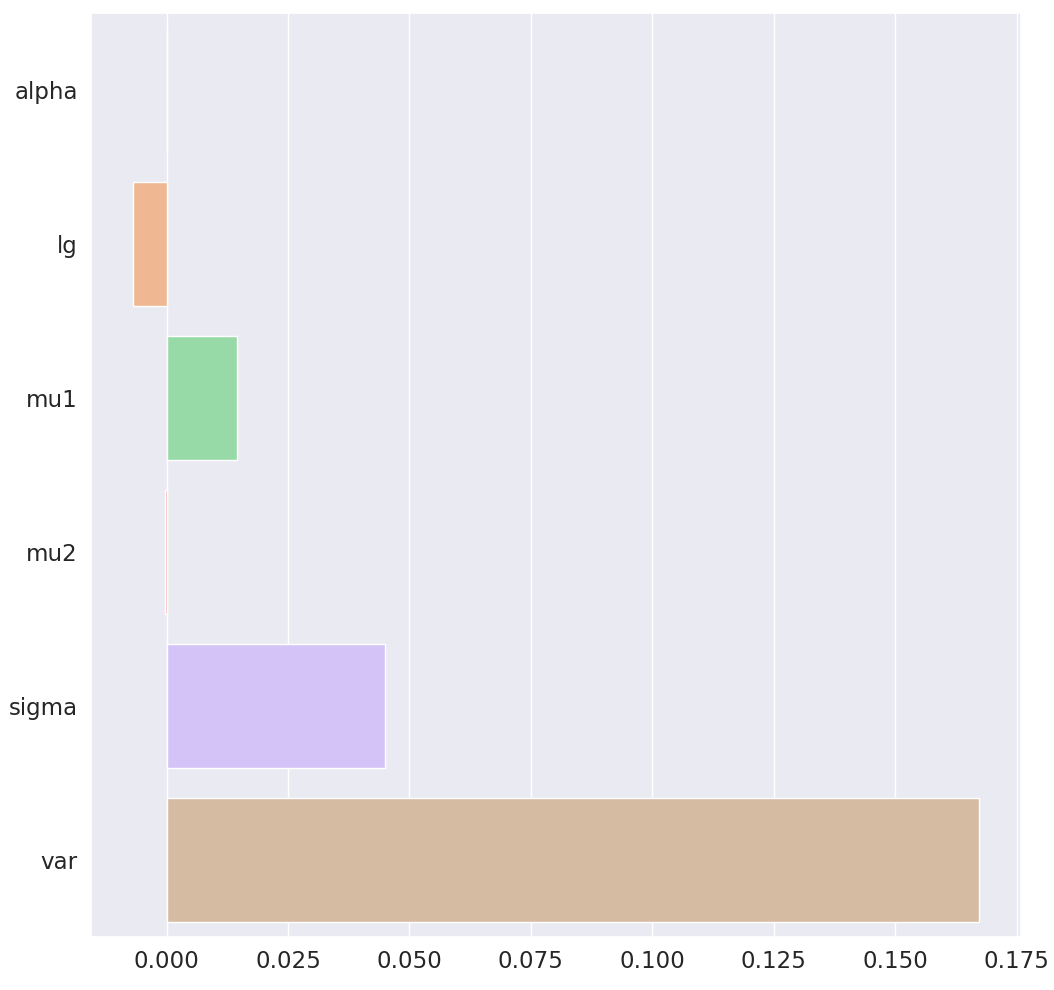
\includegraphics[scale=0.4]{feat_lr.png}
	\caption{Значимость признаков для LinearRegression}
	\label{feat_lr}
\end{figure}
На рисунке \ref{feat_lr} видно, что для алгоритма LinearRegression значимыми признаками являются задержка заявок на орбите и коэффициент вариации входящего потока. В меньшей степени является значимой интенсивность обслуживания входящий заявок, и отрицательно сказывается на результате работы наличие признака lg.
\begin{figure}[H]
	\centering
	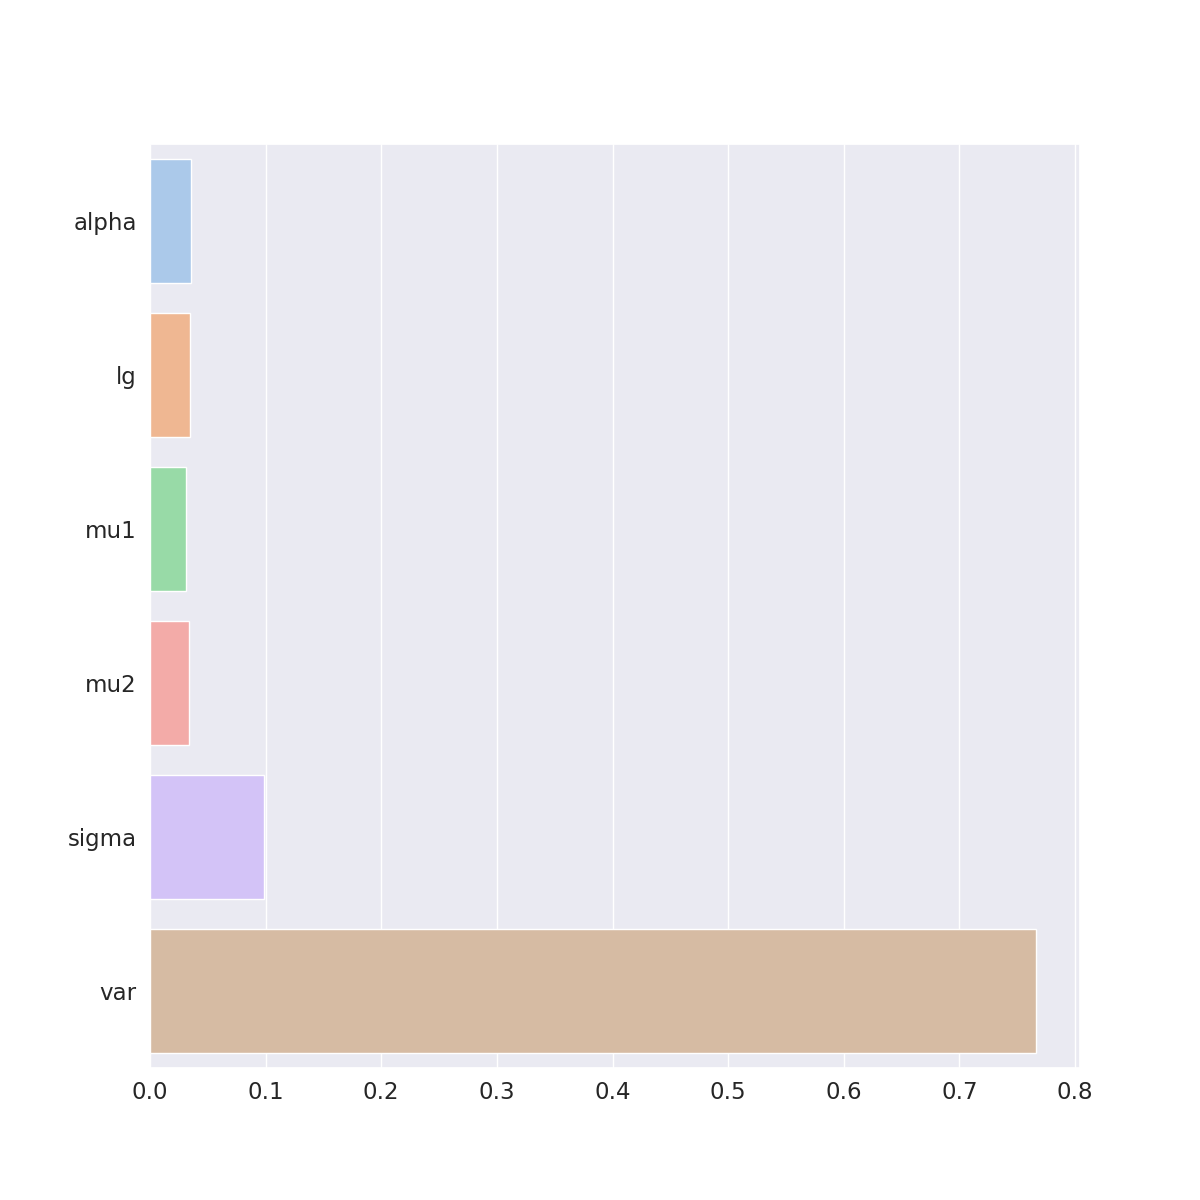
\includegraphics[scale=0.4]{feat_rf.png}
	\caption{Значимость признаков для RandomForest}
	\label{feat_rf}
\end{figure}
На рисунке \ref{feat_rf} можно наблюдать, что для алгоритма RandomForest наиболее значимыми оказались также вариация входящего потока и задержка заявок на орбите.
\begin{figure}[H]
	\centering
	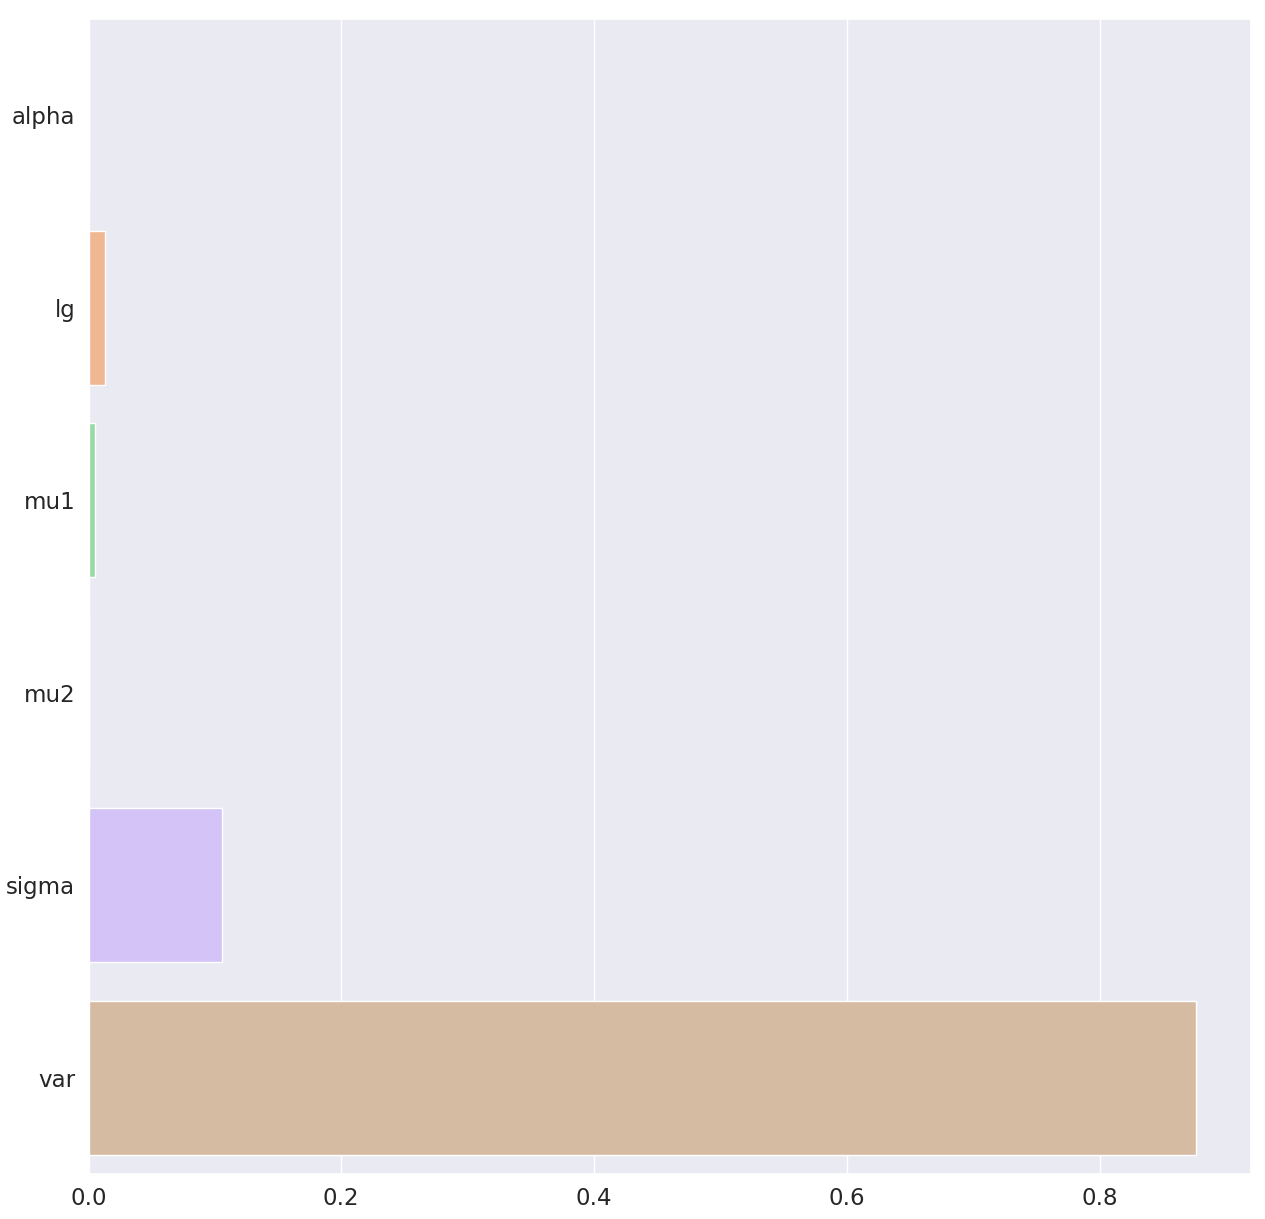
\includegraphics[scale=0.3]{feat_gb.png}
	\caption{Значимость признаков для GradientBoost}
	\label{feat_gb}
\end{figure}
\begin{figure}[H]
	\centering
	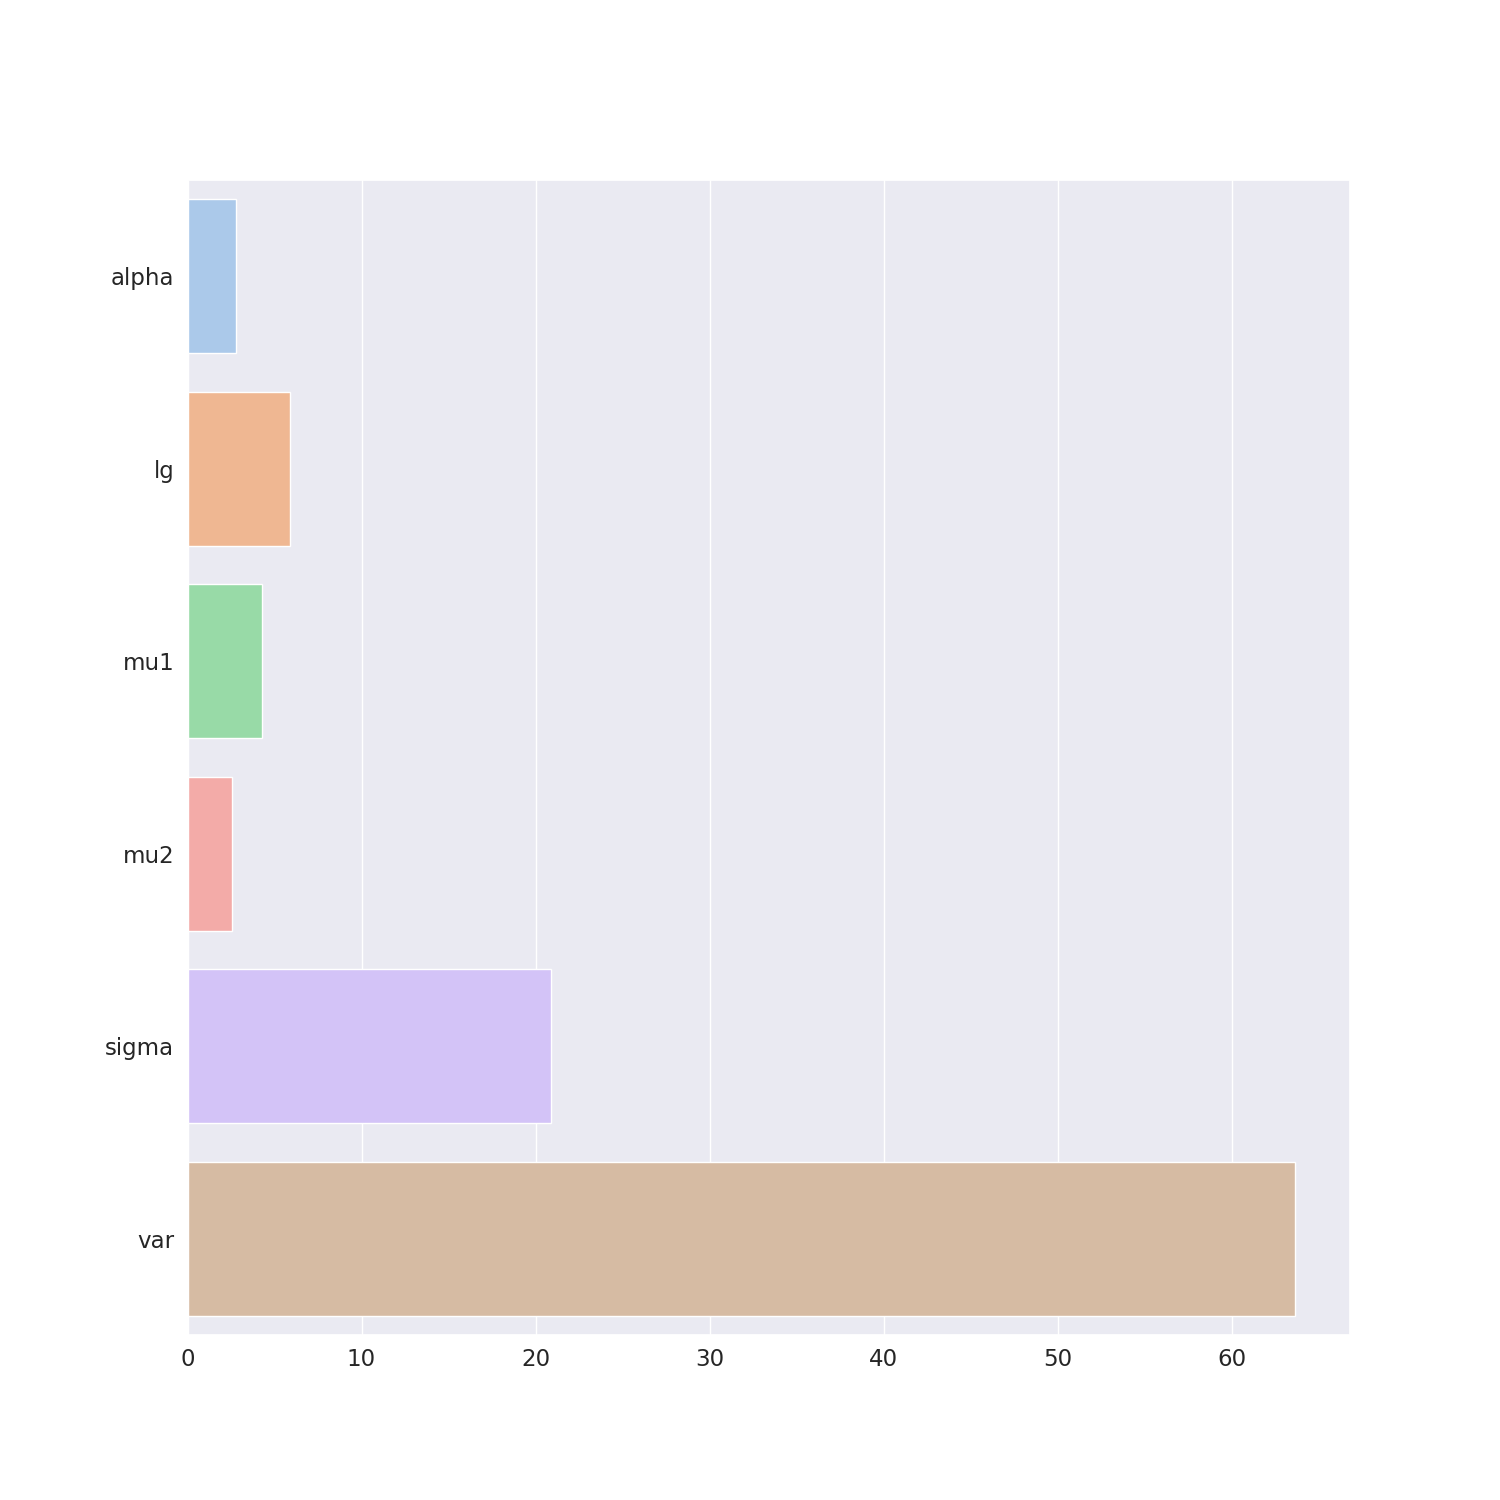
\includegraphics[scale=0.3]{feat_cb.png}
	\caption{Значимость признаков для CatBoost}
	\label{feat_cb}
\end{figure}
%райангослингсупермужик.написала я.
%леди гага гагагагагага.
%я хочу пивооо.
%хто я.
%зеленский... мое старческое многоточие. я не знаю что тебе сказать. что за взгляд. я тебя сбил. я люблю пиво. че котопес отменяется?:) что хочешь то пиши как видищб в дипломе этого нет што нет? тань...не знаю что тебе предложить? это пайин. господи какая же ты встратая когда пьяная. то двойник то што... нинаю.хахахахахахаах - сказал Леша. аха. опопопопоп
Для алгоритмов GradientBoost и CatBoost значимыми признаками также выступают sigma и var. Основываясь на полученных данных, оставим в обучающей выборке для каждой модели только значимые признаки.

Задание гиперпараметров алгоритмов \cite{feurer2019hyperparameter} будем производить случайным подбором в 5 итераций при помощи алгоритма scikit-learn RandomizedSearchCV. Важно заметить, что из тестовой выборки не выделялась валидационная, так как RandomizedSearchCV содержит встроенную кросс-валидацию. Он позволяет, начиная с указанных начальных значений, итеративно подобрать оптимальные гиперпараметры для модели. Для метода наименьших квадратов эта процедура не производится, поскольку метод не допускает задания каких-либо параметров.
\begin{pyin}[rand_forest_param]
rf = RandomForestRegressor(n_jobs=-1)
parameters_rf = {'n_estimators': range (100,150, 10),
'criterion':  ['squared_error'],
'max_depth' : range(1,9,1),
'min_samples_split': range(2,30,5),
'min_samples_leaf':range(1,30,5)
}
search_rf = RandomizedSearchCV(rf, parameters_rf,n_jobs=-1, n_iter = 5)
search_rf.fit(x_train_rf, y_train)
search_rf.best_params_, search_rf.best_score_
\end{pyin}
\begin{pyprint}
({'n_estimators': 110,
'min_samples_split': 2,
'min_samples_leaf': 26,
'max_depth': 7,
'criterion': 'squared_error'},
0.7699992121816944)
\end{pyprint}
\begin{pyin}[random_forest_learn]
best_model_rf = search_rf.best_estimator_
best_model_rf.fit(x_train_rf, y_train)
y_pred_test_rf = best_model_rf.predict(x_test_rf)

print('MAE:', mean_absolute_error(y_test, y_pred_test_rf))
print('RMSE:', mean_squared_error(y_test, y_pred_test_rf, squared=False))
print('R2_score:', r2_score(y_test, y_pred_test_rf))
\end{pyin}
\begin{pyprint}
MAE: 0.06538199710376982
RMSE: 0.09781859274247506
R2_score: 0.7695224558769049
\end{pyprint}
В ячейке \ref{rand_forest_param} производится задание начальных значений гиперпараметров для алгоритма случайных деревьев. Среди параметров:
\begin{itemize}
	\item n\_estimators --- количество деревьев решений.
	\item criterion --- методы оценки ошибки в процессе обучения. По умолчанию выбрано среднеквадратическое отклонение.
	\item max\_depth --- максимальная глубина дерева.
	\item min\_samples\_split --- минимальное количество сэмплов, требуемое для расщепления вершины дерева.
	\item min\_samples\_leaf --- минимальное количество сэмплов, требуемое для превращения вершины в лист.
\end{itemize}
Далее производится подбор параметров алгоритма, дающих максимальную точность, измеряемую коэффициентом детерминации. Коэффициент детерминации является основной метрикой качества для решений задач регрессии \cite{gomar2011validation}. В данном случае, он составил 0.769.
В ячейке \ref{random_forest_learn} производится обучение модели с лучшими гиперпараметрами и оценка точности, которая проводится при помощи следующих метрик:  средняя абсолютная ошибка (MAE), среднеквадратическое отклонение (RMSE) и коэффициент детерминации (R2\_score).

Для остальных моделей использовалась та же последовательность операций. В итоге, были получены следующие результаты
\begin{figure}[H]
	\centering
	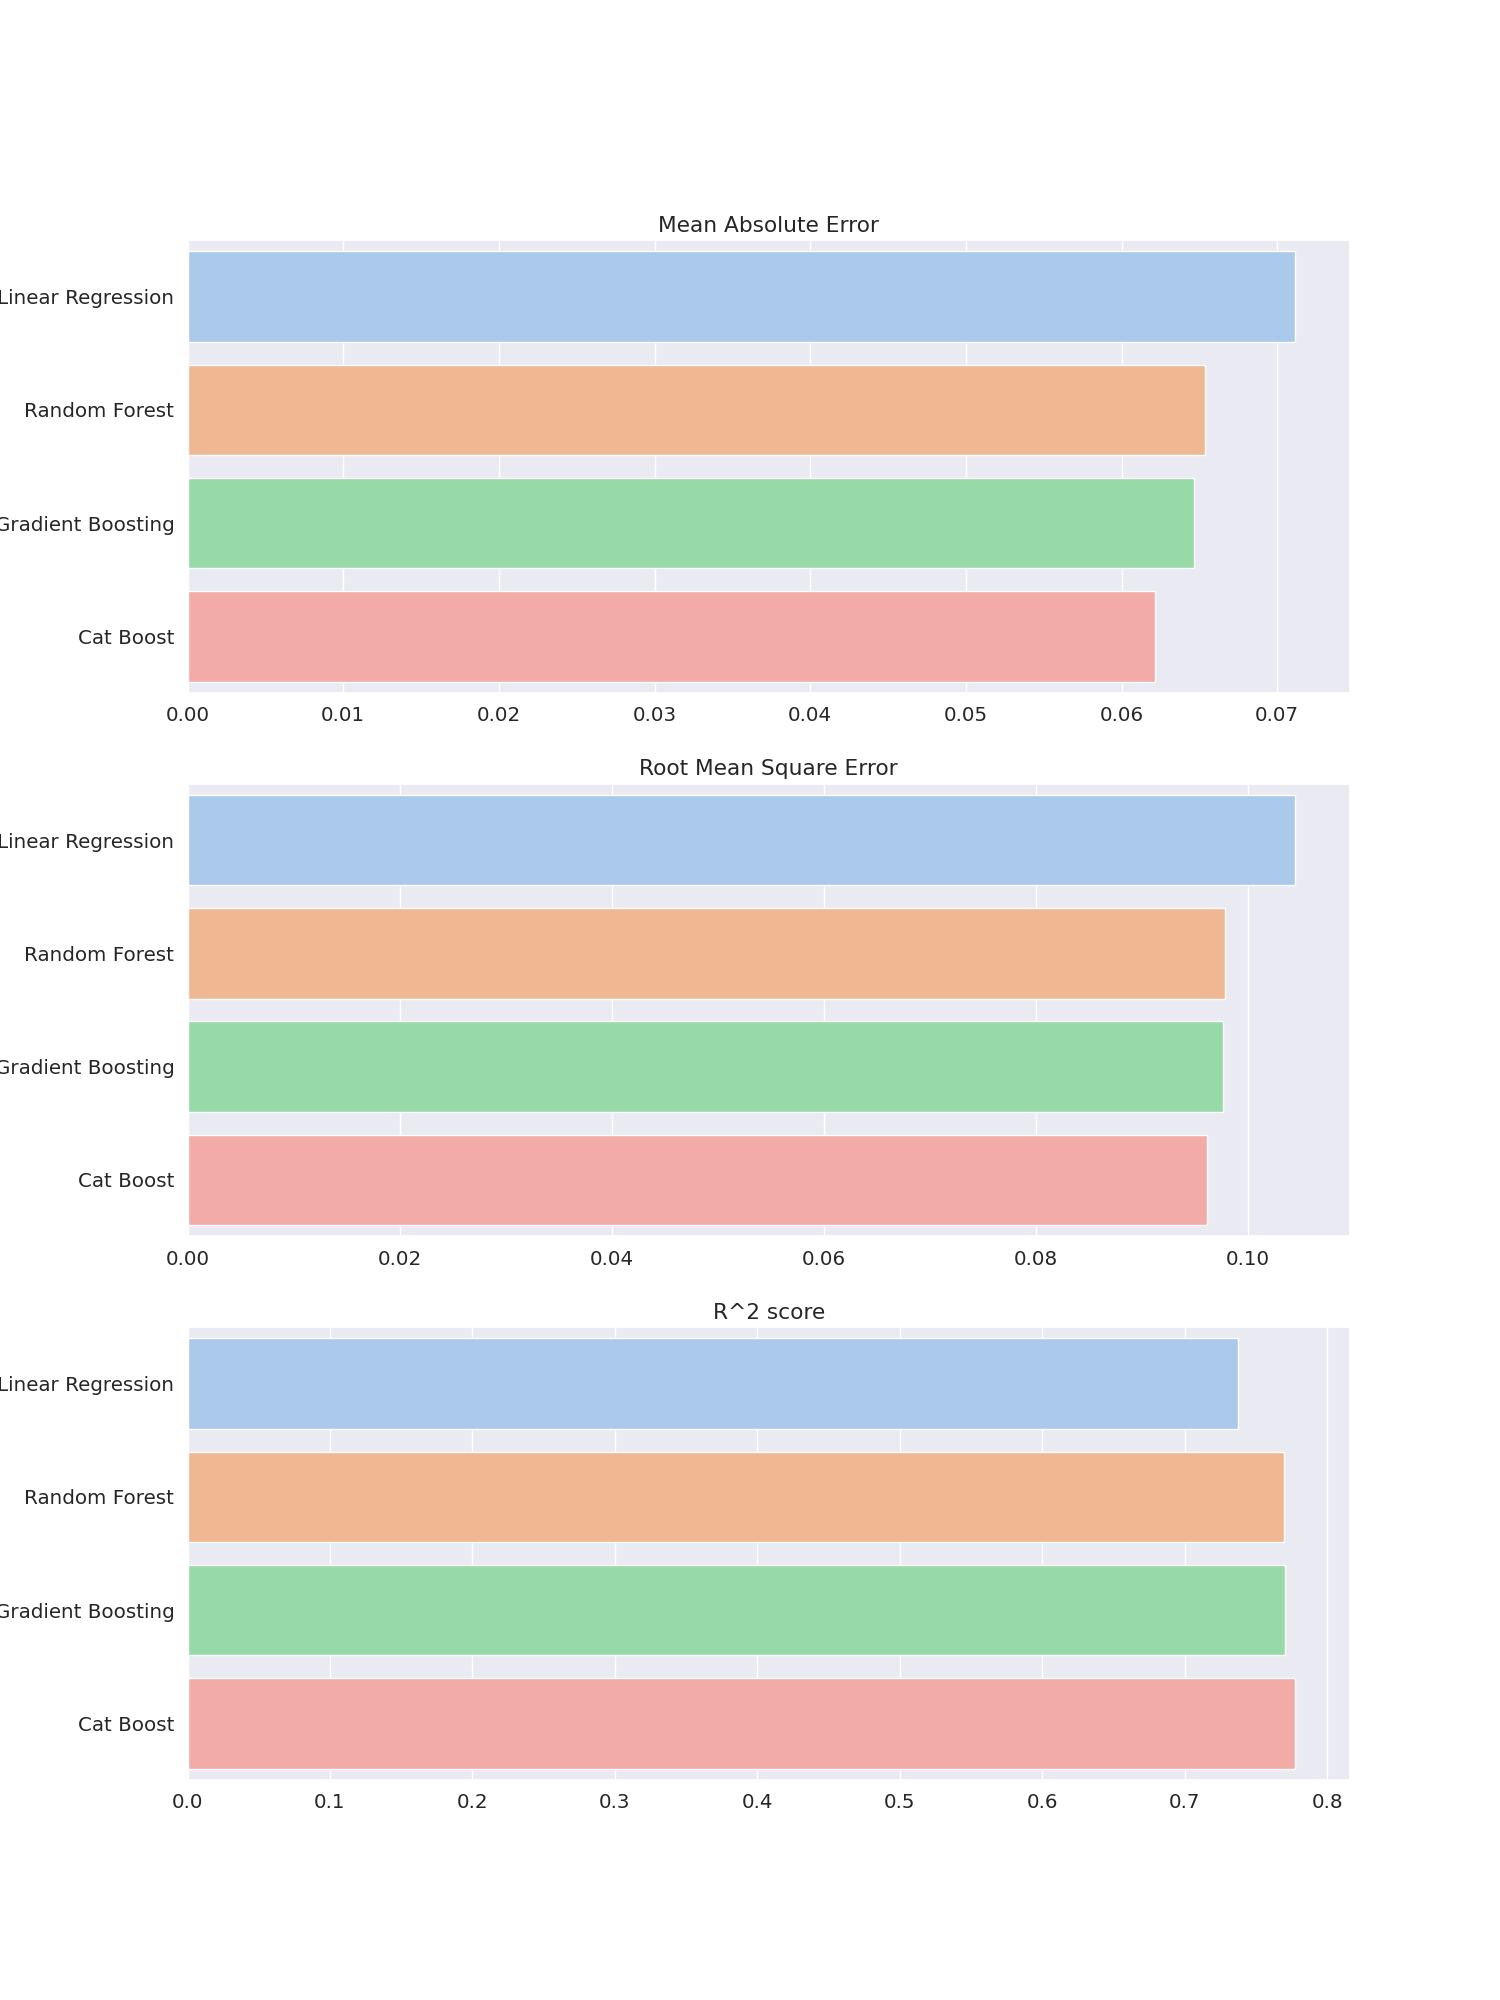
\includegraphics[scale=1,width=\textwidth]{model_accuracy.png}
	\caption{Оценка точности моделей}
	\label{model_accuracy}
\end{figure}
\begin{figure}[H]
	\centering
	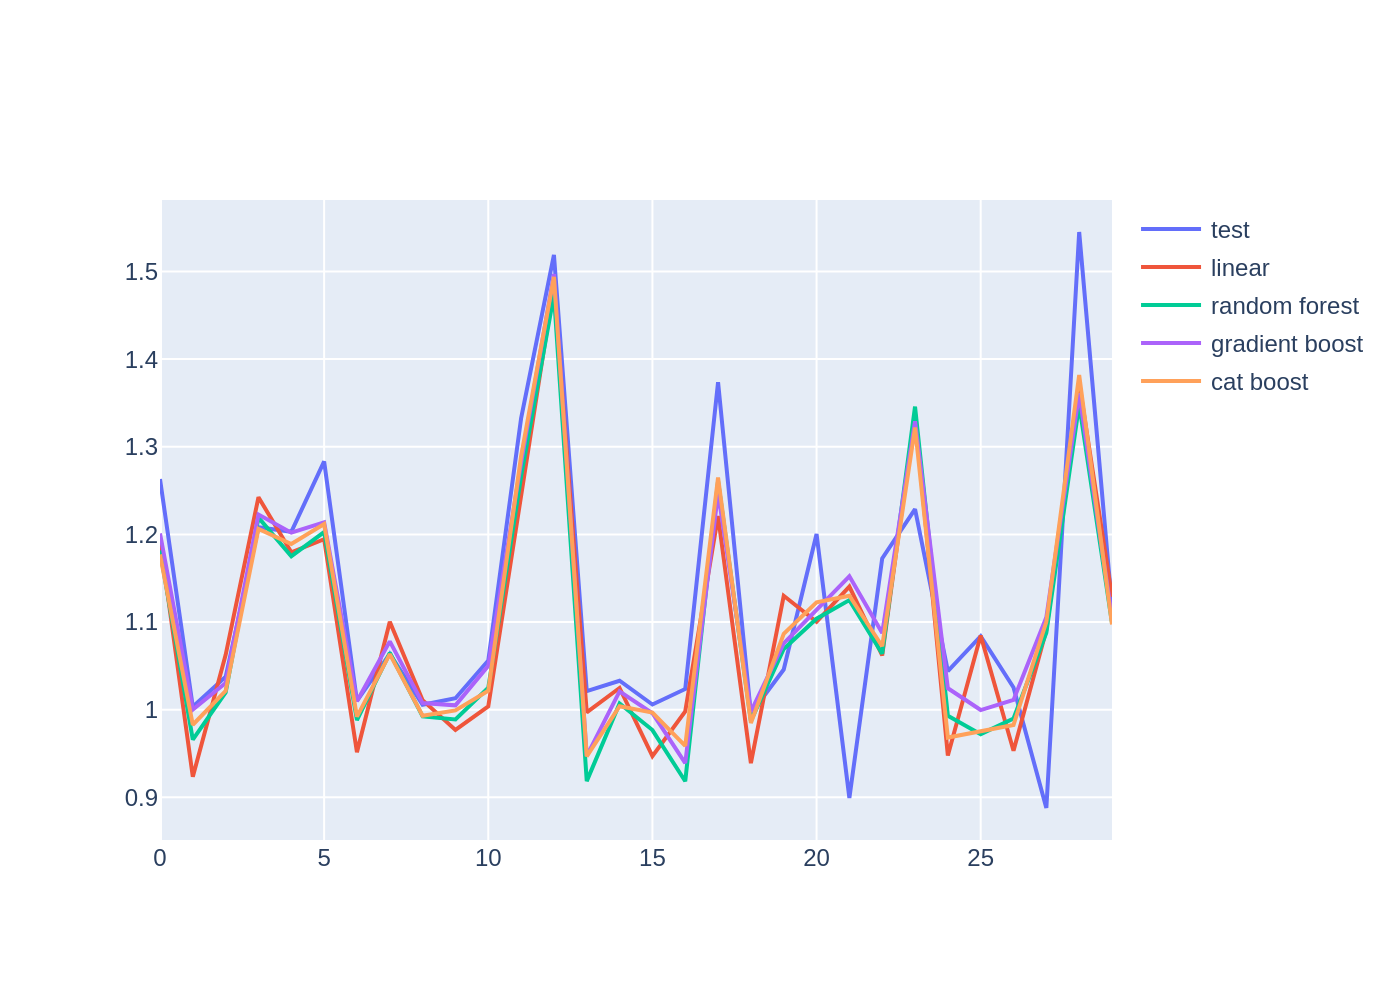
\includegraphics[scale=1,width=\textwidth]{pred_example.png}
	\caption{Сравнение предсказаний моделей}
	\label{pred_example}
\end{figure}
Как видно на рисунке \ref{model_accuracy}, CatBoost оказался самым точным среди выбранных алгоритмов --- результаты его предсказаний имеют наименьшую среднюю абсолютную и квадратические ошибки и наибольшее значение коэффициента детерминации, равное 0.774. Рассмотрение результатов предсказаний в целом показывает, что общая точность моделей находится в районе 80\%. Для апробирования подхода данный результат является в достаточной степени приемлемым. Также, можно предложить, почему точность моделей не оказалась выше: на рисунке \ref{pred_example} представлен отрезок тестового вектора значения коэффициента вариации выходящего процесса с наложением на него предсказаний. Можно заметить, что для значений, которые наиболее приближены к среднему по выборке, предсказания точны, однако для менее частых модели не смогли дать верный ответ. Это обусловлено слабой дисперсией в распределении значимых признаков в выборке (таблица \ref{table_feature_distr}), что приводит к переобучению моделей на определенном диапазоне значений признаков, делая предсказания для остальных случаев искаженными. Для улучшения качества предсказаний требуется изменить метод генерации параметров таким образом, чтобы признаки были распределены более равномерно и охватывали как можно больше возможных значений.